\subsection{Pump profile dependent temperature increase on gain surface}

With the concepts described in
appendix~\ref{app:comsol_deriv}
and section~\ref{sec:comsol:beamprofile}
we can look at
the expected temperature increase
of our structure,
corresponding to different pump beam profiles.
The thermal load
inflicted on the structure
depends on this pump distribution.
The image of a multi-mode fiber
can be described by a super-Gaussian.
This category describes
a generalized Gaussian profile
of the form $f(x)\sim\e^{-|\frac{x}{w}|^\beta}$
\cite{Chernikov2010},
see Fig.~\ref{img:visuallize_sGauss}.
It covers
distributions between
Gaussian ($\beta=2$) and flat-top ($\beta=\infty$).
The closer the pump beam distribution
resembles a flat-top distribution,
the more evenly the temperature load
is distributed.

The numerical analysis
for super-Gaussian profiles
is particularly interesting:
while the temperature profile
caused by Gaussian and flat-top distributions
were already reported \cite{Kemp2005},
the intermediate super-Gaussian profile
was ignored thus far.
The fact that
the pump profile
is relevant
for the performance of VECSELs
was demonstrated in \cite{Chernikov2010}.

We can assume roll over occurs
once the gain material exceeds
a critical temperature \cite{Heinen2012},
see section~\ref{sec:rth}.
In order to postpone
the critical pump power
to higher values,
we have to lower the peak temperature
invoked by the pump.
Figure~\ref{img:Comsol_Tvsr} shows,
this can be achieved
by either assuming
a super-Gaussian beam profile
or a regular Gaussian
with larger spot size.

\begin{figure}
\centering
\subfigure{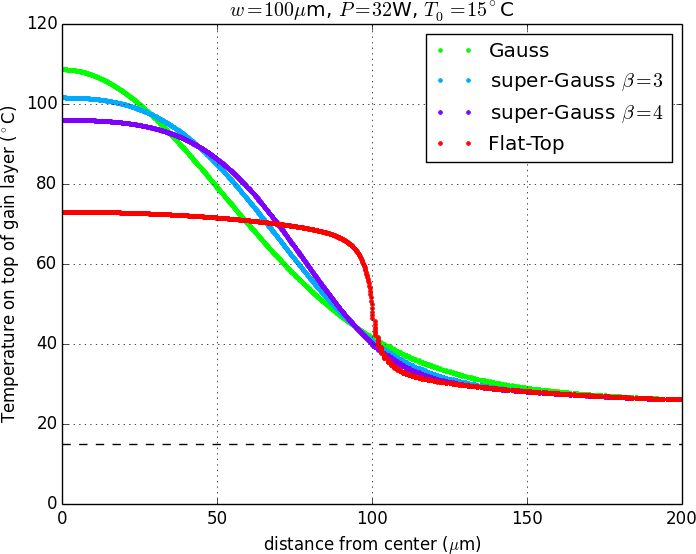
\includegraphics[width=7cm]{img/Comsol_Tvsr_32W_100um.png}}
\subfigure{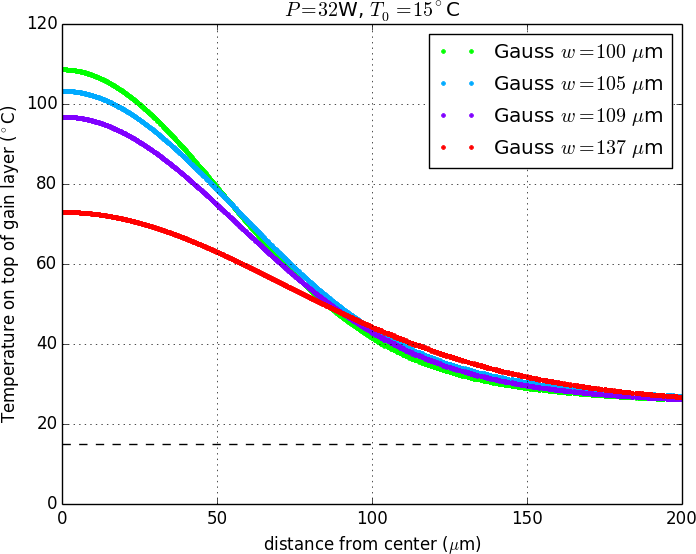
\includegraphics[width=7cm]{img/Comsol_Tvsr_32W_sG-equivs.png}}
\caption{Temperature along surface of the gain section, $z_\mathrm{0g}$
(Tab.~\ref{tab:comsolparams}).
The different beam shapes from Fig.~\ref{img:visuallize_sGauss}
with the same total power
induce a different increase in temperature
with respect to $T_0$,
indicated by the dashed line (left).
The same peak temperature can be found
employing regular Gaussians
with larger beam spots.
These however,
have a larger fraction
of the power distribution
below threshold
in the tail region,
which contributes only to heating
but no light emission.}
\label{img:Comsol_Tvsr}
\end{figure}

The peak temperature
is not the only relevant quantity
for an efficient pump profile:
the gain needs to be irradiated
with enough power
to transcend threshold.
The regions of the sample
irradiated by pump light
but below threshold
do not contribute to the laser output.
However, these regions do heat the structure.

The stronger we pump,
the larger the area on the sample
irradiated by above-threshold power.
This above-threshold
region corresponds to
the relevant, effective area.
In the case of the accentuated Gaussian beam,
the center exceeds
the roll over temperature
at a relatively low pump power,
while the effective area
is still relatively small.
In contrast,
a super-Gaussian pump profile
is capable activating
a larger effective area,
while at the same time
lowering the peak temperature.
Consequentially,
roll over is expected
to occur at higher pump power.

These simulations demonstrate
the thermal management
depends on the pump profile.
Furthermore, they suggest
a Gaussian pump profile
to be non-ideal
concerning the inflicted thermal load.
This reasoning is consistent
with the findings in \cite{Chernikov2010}.

This provokes
me to issue a warning:
extracting thermal resistance $\Rth$
only for the hottest spot,
as suggested in section~\ref{sec:rth},
does not tell the full story.
We can find normal Gaussians
with the same peak temperature
as super-Gaussians,
Fig.~\ref{img:Comsol_Tmax_BeamProfile}.
Comparing thus extracted values of $\Rth$
with values measured with other setups --
and expectedly different pump profiles --
is hence not valid.

\begin{figure}
\centering
\subfigure{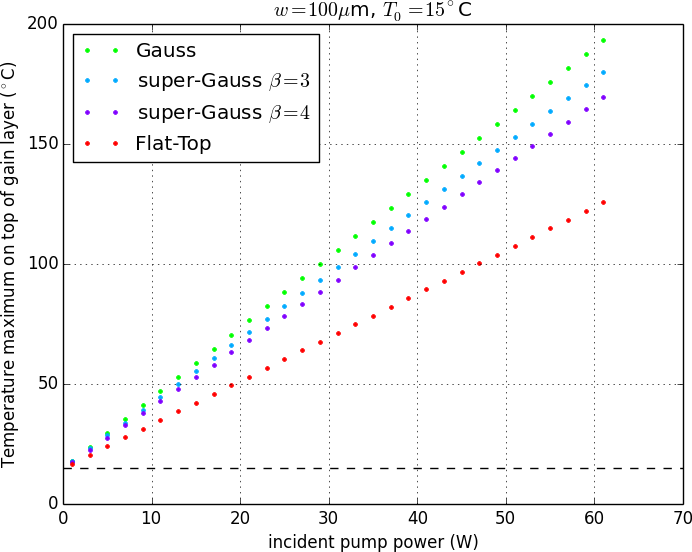
\includegraphics[width=7cm]{img/Comsol_Tmax_BeamProfile_32W_100um.png}}
\subfigure{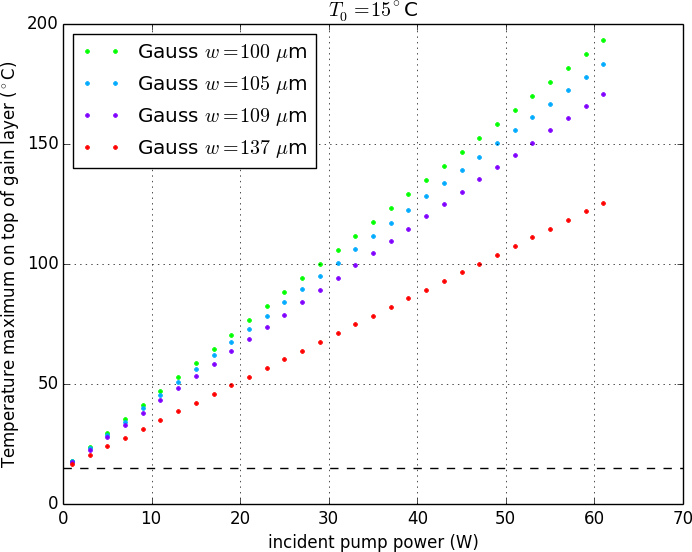
\includegraphics[width=7cm]{img/Comsol_Tmax_BeamProfile_32W_sG-equiv.png}}
\caption{The maximum temperature (i.e. at $r=0\,\mu\mathrm{m}$)
of the different beam profile depicted in Fig.~\ref{img:Comsol_Tvsr},
for various settings of total power.
The increase in peak temperature
does not change qualitatively
whether we consider super-Gaussians (left)
or regular Gaussians with larger radii (right).}
\label{img:Comsol_Tmax_BeamProfile}
\end{figure}
